\section{SONCEBOZ BLDC-Motor (CPM90 5934)}
Der SONCEBOZ BLDC-Motor CPM90 ist ein kleiner BLDC-Motor, der mit maximal 48V versorgt wird, er kann auch mit niedrigeren Spannungsniveaus betrieben werden. Deshalb ist er passend als Testmaschine für den Motorprüfstand. Au{\ss}erdem hat dieses Modell eine integrierte CAN-Bus Ansteuerung, was die Gestaltung der Ansteuerung um vieles leichter macht. \cite{SONCEBOZ}
Dieser BLDC-Motor ist auf der Testbank mechanisch verbaut und für ihn muss eine Software geschrieben werden. 


\begin{figure}[h]
    \begin{center}
        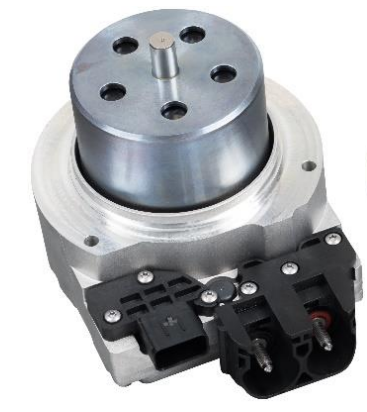
\includegraphics[width=6.68cm, height= 7.5cm]{images/Abbildung 3.png}
        \caption{SONCEBOZ BLDC-Motor CPM90 5934 \cite{SONCEBOZ}}
        \label{SONCEBOZ BLDC}
        \end{center}
\end{figure}
\clearpage
\subsection{Technische Daten}

\begin{table}[ht]
    \centering
    \begin{tabular}{|l | r|} 
        \hline
        Leistung & 5,4kW\\
        \hline
        Drehmoment & 14,2Nm\\
        \hline
        Drehzahl & 600 min$^-$$^1$ \\
        \hline
        Kommunikation & CAN\\
        \hline
        Gewicht & 4,1kg\\
        \hline
        Dimensionen & \emptyset 88,57 x 2.62mm\\
        \hline
        Versorgungsspannung & 48VDC\\
        \hline
    \end{tabular}

    
    \caption{Technische Daten des SONCEBOZ BLDC-Motors \cite{SONCEBOZ}}
    \label{table::tDaten}
\end{table}

\subsection{Funktionsdiagramm und PIN-Belegung}
\begin{figure}[h]
    \begin{center}
        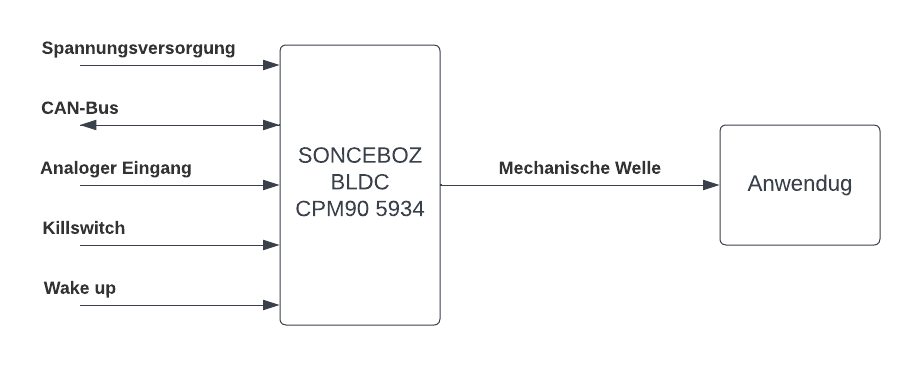
\includegraphics[width=14.61cm, height= 5.79cm]{images/Abbildung 4.png}
        \caption{Funktionsdiagramm des SONCEBOZ BLDC-Motors \cite{SONCEBOZ}}
        \label{Fdiagramm SONCEBOZ BLDC}
        \end{center}
\end{figure}
\clearpage

\begin{table}[ht]
    \begin{center}
    \begin{tabular}{|c | l | l|} 
        \hline
        Pin Nummer & Zuordnung & Kommentar\\
        \hline
        1 & CAN\_L & CAN Low\\
        \hline
        2 & D\_IO\_1 & nicht benutzt \\
        \hline
        3 & CAN\_H & CAN High\\
        \hline
        4 & DGND & nicht benutzt\\
        \hline
        5 & Wake up & Logik aktivieren\\
        \hline
        6 & 5V\_IO & 5V Versorgung für Kill Switch\\
        \hline
        7 & Killswitch & Power Stage aktivieren\\
        \hline
        8 & 5V\_1 & 5V Versorgung für Analog1\_\\
        \hline 
        9 & AN\_1 & Signal Eingang für Analog\_1\\
        \hline 
        10 & A\_GND\_1 & GROUND für Analog\_1\\ 
        \hline
        11 & 5V\_2 & 5V Versorgung für Analog\_2\\
        \hline 
        12 & AN\_2 & Signal Eingang für Analog\_2\\
        \hline  
        13 & A\_GND\_2 & GROUND für Analog\_2\\
        \hline
        14 & 5V\_3 & 5V Versorgung für Analog\_3\\
        \hline 
        15 & AN\_3 & Signal Eingang für Analog\_3\\
        \hline 
        16 & A\_GND\_3 & GROUND für Analog\_3\\
        \hline
    \end{tabular}

    \label{table::PIN-Belegung}
    
    \caption{PIN-Belegung des SONCEBOZ BLDC-Motor \cite{SONCEBOZ}}
\end{center}
\end{table}

Spannungsversorgung:
\begin{itemize}
    \item Die Hauptspannungsversorgung ist auf dem PIN U$_{bat+}$ und dem PIN U$_{bat-}$ des BLDC-Motors, dieser wird mit einem 24V Netzteil versorgt, bei dem zwei Ausgänge in Serie geschalten wurden.  \cite{SONCEBOZ}
\end{itemize}

CAN-Bus:
\begin{itemize}
    \item Der CAN-BUS wird bei den beiden PINs CAN\_L und CAN\_H angeschlossen und dann mit der SPS verbunden, worüber der BLDC-Motor gesteuert wird und verschiedene Informationen vom Motor zur SPS geschickt werden. \cite{SONCEBOZ}
\end{itemize}

Analoge Eingänge:
\begin{itemize}
    \item 
    Die PINs AN\_1, AN\_2 und AN\_3 werden mit maximal 5V versorgt und auf PIN A\_GND\_1, 2 oder 3 auf Masse gelegt. 
    Diese Analogen Signal-Eingänge werden an den Ausgang von externen Sensoren geschlossen, um den Mikrocontroller diese Signale zu senden, 
    dieser wandelt diese Signale um und regelt damit den Motor, falls eine Regelung implementiert wurde, oder gibt die Signale über die CAN-Schnittstelle aus. \cite{SONCEBOZ}
\end{itemize}

Analoge Ausgänge:
\begin{itemize}
    \item Die PINs 5V\_1, 5V\_2 und 5V\_3 werden verwendet, um externe Sensoren zu versorgen. Diese werden auf den jeweiligen PIN A\_GND\_1, 2 oder 3 auf Masse gelegt. In dem Blockschaltbild der Platine ist ersichtlich, dass diese Ausgänge durch die Hauptspannungsversorgung gespeist werden. \cite{SONCEBOZ}
\end{itemize}

Killswitch:
\begin{itemize}
    \item Dieser Schalter hat die Funktion den Motor komplett von der Spannung zu nehmen, er dient also als NOT-Halt. Er ist auf dem PIN 5V\_IO mit 5V versorgt und auf dem PIN Killswitch wird er ausgelöst und somit wird der Motor zum Stillstand gebracht. \cite{SONCEBOZ}
\end{itemize}

Wake up:
\begin{itemize}
    \item Dieser Schalter wird benutzt um die gesamte Spannungsversorgung ein- bzw. auszuschalten. Also dient er unter anderem als NOT-Aus. Das Öffnen dieses Schalters hat jedoch zur Folge, dass auch der Mikrocontroller spannungsfrei wird und somit keine RAM-Erinnerung erhalten bleibt.  \cite{SONCEBOZ}
\end{itemize}

\clearpage
\subsection{Blockschaltbild und Bauteilbeschreibung}

\begin{figure}[h]
        \begin{center}
            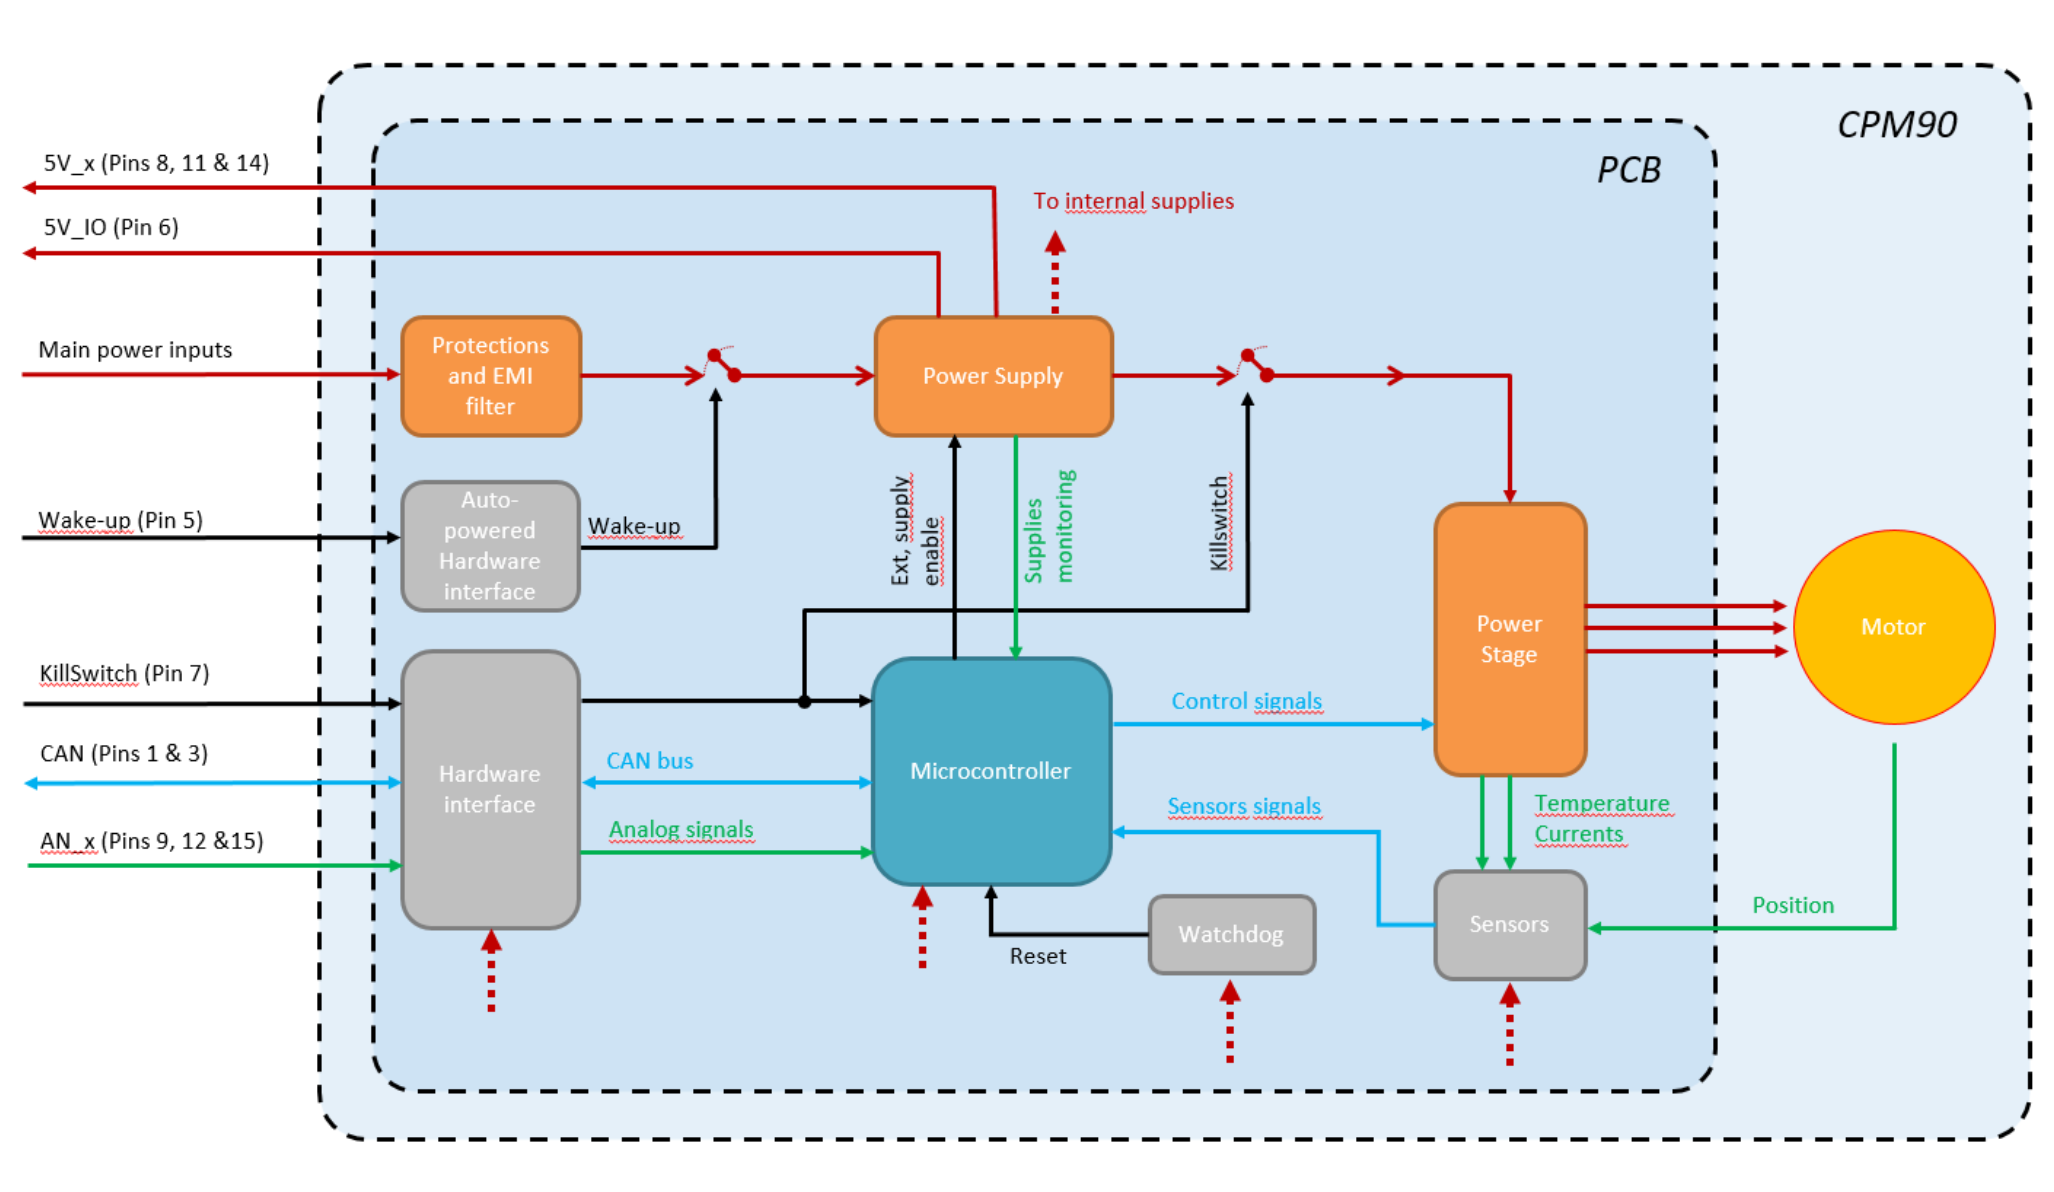
\includegraphics[width=15.76cm, height= 9.15cm]{images/Abbildung 5.png}
            \caption{Blockschaltbild der Elektronik des SONCEBOZ BLDC-Motor \cite{SONCEBOZ}}
            \label{Blockschaltbild BLDC}
            \end{center}
    \end{figure}

Das Blockschaltbild in Abbildung 5 gibt die verschiedenen Komponenten und Signalpfade auf dem Printed Curcuit Board (PCB) des SONCEBOZ BLDC-Motormodells CPM90 an. \\

Die roten Pfeile symbolisieren die verschiedenen Spannungsversorgungen, die ersten zwei sind die Versorgungen für externe Sensoren, der dritte Pfeil von oben ist die Hauptspannungsversorgung für den Motor. 
Die schwarzen Pfeile geben den Weg von Wake up und Killswitch an und die jeweiligen Schalter. 
Die blauen Pfeile zeigen die Wege der CAN-Signale an. Diese werden im Mikrocontroller verarbeitet und steuern den Motor. Au{\ss}erdem geben die Sensoren, die die Position des Motors erfassen ein CAN-Signal an den Mikrocontroller weiter das ausgelesen werden kann. Mit diesem Signal ist es beispielsweise möglich die Drehzahl ausgeben zu lassen.
Die grünen Pfeile sind analoge Ausgänge der externen Sensoren, die im Mikrocontroller verarbeitet werden. \cite{SONCEBOZ}\\


EMV Filter:
\begin{itemize}
    \item Der EMV-Filter wird verwendet, um Störungen von nahegelegenen Kapazitäten und Induktivitäten zu unterdrücken, au{\ss}erdem hilft er dabei andere Geräte nicht zu beeinflussen. \cite{SONCEBOZ}
\end{itemize}

Spannungsversorgung:
\begin{itemize}
    \item Von diesem Punkt werden alle Geräte auf der Platine versorgt. \cite{SONCEBOZ}
\end{itemize}

Leistungsstufe:
\begin{itemize}
    \item Die Leistungsstufe erhält Signale von dem Mikrocontroller und steuert passierend auf diesen den Motor. \cite{SONCEBOZ}
\end{itemize}

Selbstversorgte-Hardware-Schnittstelle:
\begin{itemize}
    \item Diese Schnittstelle ist vorhanden um den Wake up Schalter zu steuern. \cite{SONCEBOZ}
\end{itemize}

Hardware-Schnittstelle:
\begin{itemize}
    \item An dieser Schnittstelle werden alle relevanten Dinge für den Mikrocontroller angeschlossen. \cite{SONCEBOZ}
\end{itemize}

\clearpage
Watchdog:
\begin{itemize}
    \item Der Watchdog ist ein digitales System, dass die gesamte Platine überwacht und notfalls die gesamte Spannungsversorgung ausschalten kann, falls es zu schweren Schäden kommen könnte. \cite{SONCEBOZ}
\end{itemize}

Sensoren:
\begin{itemize}
    \item Das sind Sensoren, die extern und intern vorhanden sein können. Interne Sensoren sind beispielsweise solche die die Rotorposition erkennen, um den Motor zu steuern. Externe Sensoren können alle möglichen Funktionen haben und werden wie bereits beschrieben von den analogen Outputs versorgt und deren Ausgang wird bei den analogen Inputs angeschlossen. \cite{SONCEBOZ}
\end{itemize}

Mikrocontroller:
\begin{itemize}
    \item Dieser steuert alle Vorgänge auf der Platine. Er steuert die Schaltvorgänge die den Motor zum Laufen bringen. Au{\ss}erdem liest er Sensoren aus und wandelt analoge Signale in digitale um. \cite{SONCEBOZ}
\end{itemize}

